\documentclass[landscape]{article}
%ss[10pt,landscape]{article}
\usepackage{multicol}
\usepackage{calc}
\usepackage{ifthen}
\usepackage[landscape]{geometry}
\usepackage{amsmath,amsthm,amsfonts,amssymb}
\usepackage{color,graphicx,overpic}
\usepackage{wrapfig}
\usepackage{hyperref}
\usepackage[shortlabels]{enumitem}
\usepackage{enumerate}



\pdfinfo{
/Title (170_cheat_sheet.pdf)
/Creator (TeX)
/Producer (pdfTeX 1.40.0)
/Author (Nate Holland)
/Subject (CS170)
/Keywords (pdflatex, latex,pdftex,tex)}

% This sets page margins to .5 inch if using letter paper, and to 1cm
% if using A4 paper. (This probably isn't strictly necessary.)
% If using another size paper, use default 1cm margins.
\ifthenelse{\lengthtest { \paperwidth = 11in}}
    { \geometry{top=.3in,left=.3in,right=.3in,bottom=.3in} }
    {\ifthenelse{ \lengthtest{ \paperwidth = 297mm}}
        {\geometry{top=1cm,left=1cm,right=1cm,bottom=1cm} }
        {\geometry{top=1cm,left=1cm,right=1cm,bottom=1cm} }
    }

% Turn off header and footer
\pagestyle{empty}

% Redefine section commands to use less space
\makeatletter
\renewcommand{\section}{\@startsection{section}{1}{0mm}%
                            {-1ex plus -.5ex minus -.2ex}%
                            {0.5ex plus .2ex}%x
                            {\normalfont\large\bfseries}}
\renewcommand{\subsection}{\@startsection{subsection}{2}{0mm}%
                            {-1explus -.5ex minus -.2ex}%
                            {0.5ex plus .2ex}%
                            {\normalfont\normalsize\bfseries}}
\renewcommand{\subsubsection}{\@startsection{subsubsection}{3}{0mm}%
                            {-1ex plus -.5ex minus -.2ex}%
                            {1ex plus .2ex}%
                            {\normalfont\small\bfseries}}
\makeatother

% Define BibTeX command
\def\BibTeX{{\rm B\kern-.05em{\sc i\kern-.025em b}\kern-.08em
    T\kern-.1667em\lower.7ex\hbox{E}\kern-.125emX}}

% Don't print section numbers
\setcounter{secnumdepth}{0}


\setlength{\parindent}{0pt}
\setlength{\parskip}{0pt plus 0.5ex}

%My Environments
\newtheorem{example}[section]{Example}
% -----------------------------------------------------------------------

\def\ci{\perp\!\!\!\perp}



\begin{document}
\raggedright
\footnotesize
\begin{multicols}{3}


% multicol parameters
% These lengths are set only within the two main columns
%\setlength{\columnseprule}{0.25pt}
\setlength{\premulticols}{1pt}
\setlength{\postmulticols}{1pt}
\setlength{\multicolsep}{1pt}
\setlength{\columnsep}{2pt}

\begin{center}
    \Large{\underline{CS 170 Cheat Sheet}} \\
\end{center}

\subsection*{Big O notation}

$ f, g \in \mathbb{N}$, $f = O(g)$ means that f grows no faster than g if $\exists c > 0$ s.t. $F(n) \leq c g(n)$ 

$ f = \Theta(g)$ means $g = O(f)$

$f = \Theta(g)$ IFF $ f = O(g) \ \& \ g = \Theta(g)$


\subsection*{Master Theorem}
Given: $T(n) = a \times T(\frac{n}{b}) + O(n^d)$

\begin{description}

\item[a)]
$O(n^d)$ if $d > log_b(a)$

\item[b)]
$O(n^dlog(n))$ if $d = log_b(a)$

\item[c)]
$O(n^{log_b(a)})$ if $d < log_b(a)$

\end{description}

\subsection*{Sorting Algorithm Runtimes}
$HeapSort \textit{ and } MergeSort \rightarrow \Theta{(n\log{n})}$

$InsertionSort \rightarrow \Omega{(n)} \textit{ to } O(n^2)$

$QuickSort \rightarrow \Omega{(n\log{n})} \textit{ to } O(n^2)$

\subsection*{Graph Algorithms}

\textbf{DFS: O(V + E)}

Guaranteed to visit every node reachable by $v$ before returning from $v$.
Can create topological sort of DAG.

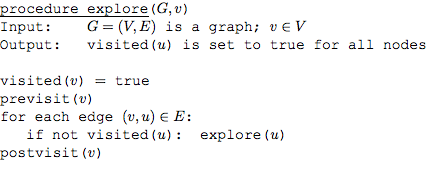
\includegraphics[scale=0.5]{DFS}

A forward edge goes to a node already in the explored set. Pre and post ordering and the edge types look like this:

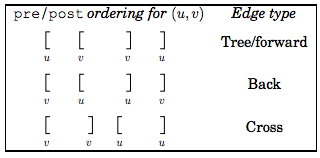
\includegraphics[scale=0.5]{prepost}

\textbf{BFS: O(V + E)}

Used to find shortest path through an unweighted graph.

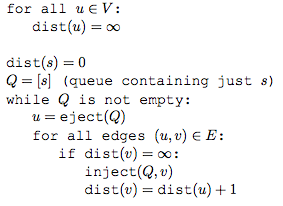
\includegraphics[scale=0.5]{BFS}

\textbf{Dijkstras: O((V + E) log V)}

Like BFS but with priority queue, used to find shortest path between two nodes on a weighted graph. Does not work with negative edge weights. 

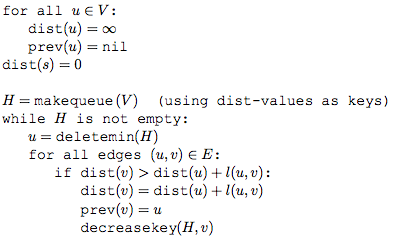
\includegraphics[scale=0.5]{dijkstra}

\textbf{Bellman Ford: O(V  E)}

Find shortest paths with negative edges as long as there are no negative cycles. Runs $V -1$ updates on all E edges. To find a negative cycle, run $V$ times, if values are updated after the $V -1$ update, there must be a negative cycle. $update()$ is harmless.

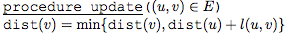
\includegraphics[scale=0.5]{BF1}

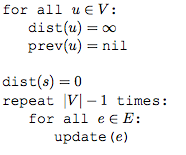
\includegraphics[scale=0.5]{BF2}

\textbf{Floyd-Warshall: $O(V^3)$}

Find the shortest path between all pairs of vertexes in a graph with positive or negative edge weights. 

\textbf{Kruskal: O(E log V)}

Use the disjoint set trees to add edges in order of increasing edge weight that doesn't complete a cycle. Used to find MST.

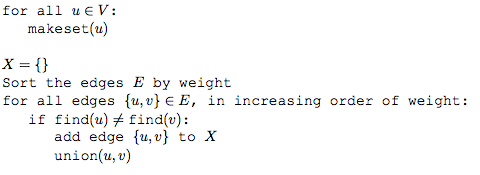
\includegraphics[scale=0.5]{kruskal}

\textbf{Prim's: O((V + E) log V)}

On each iteration, the subtree defined by X grows by one edge, namely, the lightest edge
between a vertex in S and a vertex outside S. Similar implementation as Dijkstra's. 

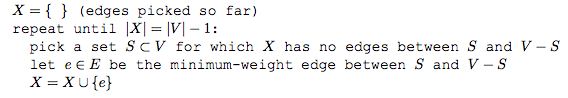
\includegraphics[scale=0.42]{prim}

\textbf{Cut Property:}
Suppose edges $X$ are part of a minimum spanning tree of
$G = (V, E)$. Pick any subset of nodes $S$ for which $X$ does not
cross between $S$ and $V-S$, and let $e$ be the lightest edge across the
partition. Then $X \cup e$ is part of some Minimum Spanning Tree.



\textbf{Huffman Encoding O(n log n) }

Make a tree of decisions of whether to pick a 0 or a 1, make all the leaves values.
Then we can follow the tree down to decode a Huffman encoding of values.

\subsection{FFT}

It is a black box which represents 2 polynomials as a list of points and then multiplies them together to create a new polynomial. Takes \textbf{O(N log N)} time. Uses roots of unity to determine where to multiply two polynomials together.

\textbf{$N^{th}$ Roots of Unity} can be found by: $ cos(\frac{2\pi j}{n}) + i \cdot sin(\frac{2\pi j}{n})$

\subsection{Dynamic Programming}

Find a recursive relationship for sub problems and then figure out the order in which we need to solve them.
Runtime can easily be deduced by the number of for loops we have to run.
Following are some basic examples of dynamic programming:

\textbf{Edit Distance: $O(n^2)$}

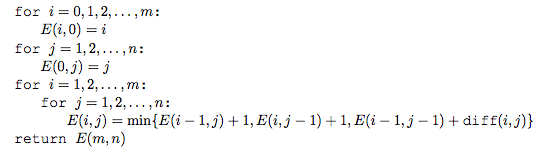
\includegraphics[scale=0.42]{edit}

\textbf{Knapsack with repetition: $O(nW)$}

K(w) is the maximum value we can achieve with weight w.

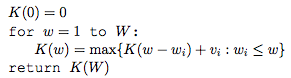
\includegraphics[scale=0.5]{knapNR}

\textbf{Knapsack without repetition: $O(nW)$}

$K(w, j)$ = maximum value achievable using a knapsack of capacity $w$ and items $1, . . . , j$.

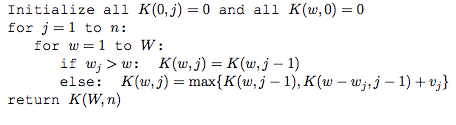
\includegraphics[scale=0.5]{knapWR}

\textbf{Longest Palindromic Subsequence: $O(n^2)$}

Takes sequence $x[1\ldots n]$ and returns the length of the longest palindromic subsequence.

For $0\leq i,j\leq n$ define $f(i,j)=$ length of the longest palindromic subsequence of $x[i\ldots j]$.  

Base case: when $i>j$ (empty string), $ f(i,j) = 0$; when $i == j$ (single character), $f(i,j) = 1$

When $i<j$, 
\[
 f(i,j) = max
  \begin{cases}
   f(i+1,j) \\
   f(i,j-1)\\
   2+f(i+1,j-1) & \text{if } x [i] = x[j]
  \end{cases}
\]

\textbf{Optimal Binary Search Tree with Probabilities:}
Let $S(i,j)$ be the cost of the cheapest tree formed by words $i$ to $j$, for $1\leq i \leq j \leq n$. Also $S(i,j) = 0$ if $i>j$.  Compute $S(i,j)$ by looking at all choices of which word to use as the root of the tree; the root could be word $k$, for any $k$ where $i\leq k \leq j$.  If $k$ is at the root, the cost of the left subtree is $S(i,k-1)$ an the right is $S(k+1, j)$.  All words need to pay one comparison at the root node and the cost of the words to the left of right can be determined recursively, so if we place work $k$ at the root, the total cost of the tree will be:

$$ \sum^k_{t=i} p_t + S(i,k-1) + S(k+1, j)$$
giving $S(i,j) = \min_{i\leq k \leq j}\{\text{the above cost}\}$

\subsection{Linear Programming}

Linear Programming is a way to state problems as systems of equations and then we can solve them in polynomial time as long as we don't need Integer Linear Programming, which is NP Complete.
It can be solved with the simplex method which we don't need to know, can just treat it like a black box.

\textbf{Remember:} when writing out your solutions make sure you add the non-negative constraints.

\subsection{Max Flow}

This is bounded by $O( C \cdot E)$ or $O ( V \cdot E^2)$

\textbf{Max-flow min-cut theorem:} the size of the maximum flow in a network equals the capacity of the smallest (s,t) cut.

\textbf{Maximum flow property:} if all edge capacities are integers, then the optimal flow found by our algorithm is integral. We can see this directly from the algorithm, which in such cases would increment the flow by an integer amount on each iteration.

When drawing the residuals make sure you draw the flow you've already used backwards, so some paths with have an arrow going forward and an arrow going backward.


\subsection{P/NP}

\textbf{P:} search problem that can be solved in polynomial time.

\textbf{NP:} search problem that can be checked to be correct in polynomial time.

\textbf{NP complete:} search problem that is at least as hard as every other NP complete problem. Basically it reduces to circuit sat, could possibly be solved in polynomial time but we doubt it.

\textbf{NP hard:} there exists NP complete Y such that Y is reducible to X but can't go the other way around. Not actually in NP.
\subsection{P/NP Basics}

\begin{center}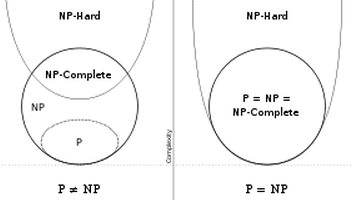
\includegraphics[scale=0.42]{complexity}\end{center}

Here are some examples of \textbf{P} and \textbf{NP} algorithms:

\begin{tabular}{| l | l |}
  \hline
  \textbf{NP} & \textbf{P} \\ \hline
  3+ SAT & 2 SAT \\ \hline
  TSP & MST \\ \hline
  Longest Path & Shortest Path \\ \hline
  3D Matching & Bipartide matching \\ \hline
  Knapsack & Unary Knapsack \\ \hline
  Independent Set & Independent Set on Trees \\ \hline
  Integer LP & Linear Programming \\ \hline
  Rudrata Path & Euler Path \\ \hline
  Balanced Cut & Minimum cut \\ \hline
\end{tabular}




\subsection{Reductions}
A search problem is NP-complete if all other search problems reduce to it.

Make sure that the conversions between the two algorithms are of polynomial size and time, otherwise the reduction does not work.

To reduce X to Y means to find a solution for X using Y.

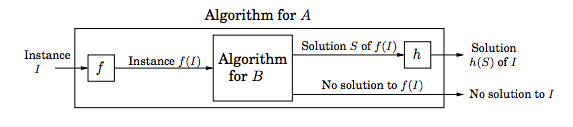
\includegraphics[scale=0.42]{reduction}	


\subsection{Dealing with NP}

There are different ways to deal with NP, one is to do intelligent but exhaustive searching.
This basically involves stopping looking at a branch as soon as we know that what we've selected won't work.
This is basically just pruning on a tree.

\textbf{Approximations}


These would be like the example where we use the MST tree to find an approximation which is at most 2 times worse than the optimal solution to the TSP problem.

There are certain classes of approximations which are as follows:

\begin{itemize}
	\item Those for which, like the TSP, no finite approximation ratio is possible.
	\item Those for which an approximation ratio is possible, but there are limits to how small
this can be. VERTEX COVER, k-CLUSTER, and the TSP with triangle inequality belong here
	\item Approximability has no limits, and polynomial approximation algorithms with error ratios arbitrarily close to zero exist. KNAPSACK resides here.
	\item Finally, there is another class of problems, between the first two given here, for which
the approximation ratio is about log n. SET COVER is an example
\end{itemize}

\textbf{Local Search Heuristics}

These can often be useful in practice but provide no guarantees for how well or how fast they will approximate the actual value.

We then deal with local optimum by using \textbf{randomization and restarts}.
This means that we will effectively run the search multiple times with different random starting points.
This gives us a better probability of finding the correct (or better) local optima.

\textbf{Simulated annealing} is another technique where we sometimes follow the optimal path, and with some random probability we actually go backwards in our search.

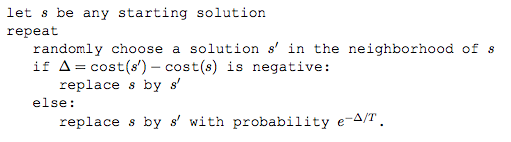
\includegraphics[scale=0.45]{annealing}

Generally we will choose our T to start large and then decrease as we go on so that with time we jump down the hills less frequently but early on we are likely to crawl out of local maximum.


\subsection{Machine Learning}

\textbf{Classification}
Let $\mathcal{Y}$ denote a set of classes. For a boolean classification, such as spam filters, $\mathcal{Y} = \{0, 1\}$. Let the observation $x \in \mathbb{R}^d$ denote a $d$-dimensional vector of features.

\textbf{K-Nearest Neighbors: $\Theta(n(d + \log k))$}

Let $x_i \ldots x_{i+k}$ be the $k$ nearest observations to $x$ from the trained set. Classify $x$ with the class with the plurality of votes from the $k$ feature vectors.

Note: for efficiency, normalize feature vectors to have the same range of values before applying k-NN. Algorithm performs worse if the dimension $d$ is too large.

\textbf{Decision Tree Inference (NP Hard)}
A $Decision Tree$ is a binary tree that represents a function $\mathbb{R}^2 \rightarrow \mathcal{Y}$ where each leaf is labeled with a decision of a classification $y \in \mathcal{Y}$. If there is an observation $x \in \mathbb{R}^2$ then we start at the root of the tree and go to the left or right child depending on the threshold value $t$. Repeat until a leaf is reached. Inference on decision trees is a greedy approach where test points in $S$ are split into $S_L$ and $S_R$ by estimating the relation of test data into similar camps (left subtrees and right subtrees). Recurse the subtrees until 

1) all remaining subtrees have the same classification

2) after a certain node depth then choose most-common class or

3) after class entropy falls beneath a threshold

\textbf{Random Forests}
A $RandomForest$ is a collection of decision trees. The goal is to reduce the error rate by classifying an observation $x$ through many decision trees and selecting the most common class as the result. Assumes each decision tree is different. Can create random  trees through either

1) Bagging (used more): train each tree on a random subset of the training set $S$. If $S$ contains $n$ test observations, then sample with replacement $n$ times to create our random subset $S^* \in S$. The expected size of $S^*$ is about 63\% the size of $S$. Use the Decision Tree Inference algorithm to construct a tree from $S^*$.

2) Feature Sampling: using a subset of $d$ features when constructing the tree. Reduces the likely hood that each tree has the same prominent feature at its root.

\rule{0.3\linewidth}{0.25pt}
\newpage
\scriptsize
\bibliographystyle{abstract}
\bibliography{refFile}
\end{multicols}
\end{document}